\problemname{\problemyamlname}

\illustration{0.2}{bomb.jpg}{
    CC BY-SA 4.0 by goff.brian on \href{https://www.vecteezy.com/vector-art/552160-bomb}{Vecteezy}
}

Oh non, il y a une bombe dans votre cuisine ! Vous devez la désamorcer avant qu'elle n'explose. Pour ce faire, vous devez résoudre un puzzle.
Vous disposez d'une grille avec $n$ lignes et $m$ colonnes. Chaque case de la grille contient une couleur. Chaque ligne contient deux flèches qui indiquent vers la droite et une autre vers la gauche.
Quand on appuie sur l'une des flèches, il y a deux cas possibles :
\begin{itemize}
    \item Si la flèche pointe vers la droite, alors toutes les couleurs de la ligne sont déplacées d'une case vers la droite.
    \item Si la flèche pointe vers la gauche, alors toutes les couleurs de la ligne sont déplacées d'une case vers la gauche.
\end{itemize}
Les lignes sont cycliques, donc si une couleur sort d'un côté de la ligne, elle rentre de l'autre côté.

Votre but est de trouver deux lignes qui sont égales après avoir entré une séquence de flèches. Si vous trouvez deux lignes qui sont égales, alors vous avez désamorcé la bombe. Si vous n'arrivez pas à trouver deux lignes qui sont égales, alors la bombe explose.

\begin{figure}[H]
    \centering
    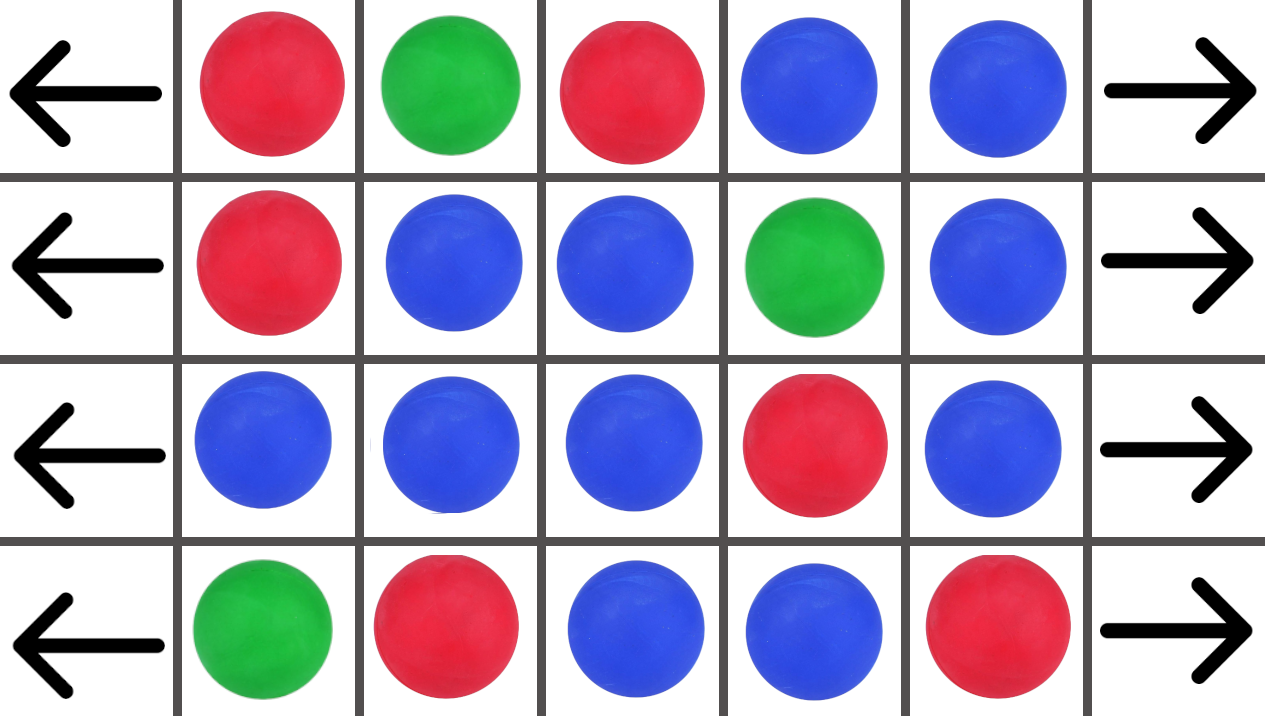
\includegraphics[width=0.5\textwidth]{illustration.png}
    \caption{Illustration de l'exemple 1}
\end{figure}

\begin{Input}
    L'entrée consiste en :
    \begin{itemize}
        \item Une ligne avec deux entiers $n$ ($0\leq n \leq 5000$), le nombre de lignes dans la grille, $m$ ($0 \leq m \leq 100$), le nombre de colonnes dans la grille.
        \item $n$ lignes avec $m$ caractères $a_{i,j}$, la couleur de la cellule $(i,j)$.
    \end{itemize}
    Il est garantis que $a_{i,j}$ est une lettre de l'alphabet \textbf{majuscule OU minuscule}.
\end{Input}

\begin{Output}
    L'indice des deux lignes dans l'ordre croissant qui sont égales. Si plusieurs lignes correspondent, affichez la paire de lignes la plus petite. S'il n'est pas possible de trouver deux lignes qui sont égales, sortez \texttt{BOOM!}.
\end{Output}
